\documentclass{lni}


%\IfFileExists{latin1.sty}{\usepackage{latin1}}{\usepackage{isolatin1}}
\usepackage[latin1]{inputenc}
% Verwenden von T1 Fonts
\usepackage[T1]{fontenc}
\usepackage[ngerman]{babel}
\usepackage{graphicx}
\usepackage{caption}
\usepackage{subcaption}
\usepackage{amsmath}
\usepackage{amssymb}
\usepackage{listings}
%\usepackage{hyperref}
\usepackage{fancyvrb}
\usepackage{color}
\usepackage{algorithmic}
\usepackage{algorithm}
\usepackage{float}

\floatstyle{ruled}
\newfloat{program}{H}{lop}
\floatname{program}{Listing}

\makeatletter
\def\PY@reset{\let\PY@it=\relax \let\PY@bf=\relax%
    \let\PY@ul=\relax \let\PY@tc=\relax%
    \let\PY@bc=\relax \let\PY@ff=\relax}
\def\PY@tok#1{\csname PY@tok@#1\endcsname}
\def\PY@toks#1+{\ifx\relax#1\empty\else%
    \PY@tok{#1}\expandafter\PY@toks\fi}
\def\PY@do#1{\PY@bc{\PY@tc{\PY@ul{%
    \PY@it{\PY@bf{\PY@ff{#1}}}}}}}
\def\PY#1#2{\PY@reset\PY@toks#1+\relax+\PY@do{#2}}

\def\PY@tok@gd{\def\PY@tc##1{\textcolor[rgb]{0.63,0.00,0.00}{##1}}}
\def\PY@tok@gu{\let\PY@bf=\textbf\def\PY@tc##1{\textcolor[rgb]{0.50,0.00,0.50}{##1}}}
\def\PY@tok@gt{\def\PY@tc##1{\textcolor[rgb]{0.00,0.25,0.82}{##1}}}
\def\PY@tok@gs{\let\PY@bf=\textbf}
\def\PY@tok@gr{\def\PY@tc##1{\textcolor[rgb]{1.00,0.00,0.00}{##1}}}
\def\PY@tok@cm{\let\PY@it=\textit\def\PY@tc##1{\textcolor[rgb]{0.25,0.50,0.50}{##1}}}
\def\PY@tok@vg{\def\PY@tc##1{\textcolor[rgb]{0.10,0.09,0.49}{##1}}}
\def\PY@tok@m{\def\PY@tc##1{\textcolor[rgb]{0.40,0.40,0.40}{##1}}}
\def\PY@tok@mh{\def\PY@tc##1{\textcolor[rgb]{0.40,0.40,0.40}{##1}}}
\def\PY@tok@go{\def\PY@tc##1{\textcolor[rgb]{0.50,0.50,0.50}{##1}}}
\def\PY@tok@ge{\let\PY@it=\textit}
\def\PY@tok@vc{\def\PY@tc##1{\textcolor[rgb]{0.10,0.09,0.49}{##1}}}
\def\PY@tok@il{\def\PY@tc##1{\textcolor[rgb]{0.40,0.40,0.40}{##1}}}
\def\PY@tok@cs{\let\PY@it=\textit\def\PY@tc##1{\textcolor[rgb]{0.25,0.50,0.50}{##1}}}
\def\PY@tok@cp{\def\PY@tc##1{\textcolor[rgb]{0.74,0.48,0.00}{##1}}}
\def\PY@tok@gi{\def\PY@tc##1{\textcolor[rgb]{0.00,0.63,0.00}{##1}}}
\def\PY@tok@gh{\let\PY@bf=\textbf\def\PY@tc##1{\textcolor[rgb]{0.00,0.00,0.50}{##1}}}
\def\PY@tok@ni{\let\PY@bf=\textbf\def\PY@tc##1{\textcolor[rgb]{0.60,0.60,0.60}{##1}}}
\def\PY@tok@nl{\def\PY@tc##1{\textcolor[rgb]{0.63,0.63,0.00}{##1}}}
\def\PY@tok@nn{\let\PY@bf=\textbf\def\PY@tc##1{\textcolor[rgb]{0.00,0.00,1.00}{##1}}}
\def\PY@tok@no{\def\PY@tc##1{\textcolor[rgb]{0.53,0.00,0.00}{##1}}}
\def\PY@tok@na{\def\PY@tc##1{\textcolor[rgb]{0.49,0.56,0.16}{##1}}}
\def\PY@tok@nb{\def\PY@tc##1{\textcolor[rgb]{0.00,0.50,0.00}{##1}}}
\def\PY@tok@nc{\let\PY@bf=\textbf\def\PY@tc##1{\textcolor[rgb]{0.00,0.00,1.00}{##1}}}
\def\PY@tok@nd{\def\PY@tc##1{\textcolor[rgb]{0.67,0.13,1.00}{##1}}}
\def\PY@tok@ne{\let\PY@bf=\textbf\def\PY@tc##1{\textcolor[rgb]{0.82,0.25,0.23}{##1}}}
\def\PY@tok@nf{\def\PY@tc##1{\textcolor[rgb]{0.00,0.00,1.00}{##1}}}
\def\PY@tok@si{\let\PY@bf=\textbf\def\PY@tc##1{\textcolor[rgb]{0.73,0.40,0.53}{##1}}}
\def\PY@tok@s2{\def\PY@tc##1{\textcolor[rgb]{0.73,0.13,0.13}{##1}}}
\def\PY@tok@vi{\def\PY@tc##1{\textcolor[rgb]{0.10,0.09,0.49}{##1}}}
\def\PY@tok@nt{\let\PY@bf=\textbf\def\PY@tc##1{\textcolor[rgb]{0.00,0.50,0.00}{##1}}}
\def\PY@tok@nv{\def\PY@tc##1{\textcolor[rgb]{0.10,0.09,0.49}{##1}}}
\def\PY@tok@s1{\def\PY@tc##1{\textcolor[rgb]{0.73,0.13,0.13}{##1}}}
\def\PY@tok@sh{\def\PY@tc##1{\textcolor[rgb]{0.73,0.13,0.13}{##1}}}
\def\PY@tok@sc{\def\PY@tc##1{\textcolor[rgb]{0.73,0.13,0.13}{##1}}}
\def\PY@tok@sx{\def\PY@tc##1{\textcolor[rgb]{0.00,0.50,0.00}{##1}}}
\def\PY@tok@bp{\def\PY@tc##1{\textcolor[rgb]{0.00,0.50,0.00}{##1}}}
\def\PY@tok@c1{\let\PY@it=\textit\def\PY@tc##1{\textcolor[rgb]{0.25,0.50,0.50}{##1}}}
\def\PY@tok@kc{\let\PY@bf=\textbf\def\PY@tc##1{\textcolor[rgb]{0.00,0.50,0.00}{##1}}}
\def\PY@tok@c{\let\PY@it=\textit\def\PY@tc##1{\textcolor[rgb]{0.25,0.50,0.50}{##1}}}
\def\PY@tok@mf{\def\PY@tc##1{\textcolor[rgb]{0.40,0.40,0.40}{##1}}}
\def\PY@tok@err{\def\PY@bc##1{\fcolorbox[rgb]{1.00,0.00,0.00}{1,1,1}{##1}}}
\def\PY@tok@kd{\let\PY@bf=\textbf\def\PY@tc##1{\textcolor[rgb]{0.00,0.50,0.00}{##1}}}
\def\PY@tok@ss{\def\PY@tc##1{\textcolor[rgb]{0.10,0.09,0.49}{##1}}}
\def\PY@tok@sr{\def\PY@tc##1{\textcolor[rgb]{0.73,0.40,0.53}{##1}}}
\def\PY@tok@mo{\def\PY@tc##1{\textcolor[rgb]{0.40,0.40,0.40}{##1}}}
\def\PY@tok@kn{\let\PY@bf=\textbf\def\PY@tc##1{\textcolor[rgb]{0.00,0.50,0.00}{##1}}}
\def\PY@tok@mi{\def\PY@tc##1{\textcolor[rgb]{0.40,0.40,0.40}{##1}}}
\def\PY@tok@gp{\let\PY@bf=\textbf\def\PY@tc##1{\textcolor[rgb]{0.00,0.00,0.50}{##1}}}
\def\PY@tok@o{\def\PY@tc##1{\textcolor[rgb]{0.40,0.40,0.40}{##1}}}
\def\PY@tok@kr{\let\PY@bf=\textbf\def\PY@tc##1{\textcolor[rgb]{0.00,0.50,0.00}{##1}}}
\def\PY@tok@s{\def\PY@tc##1{\textcolor[rgb]{0.73,0.13,0.13}{##1}}}
\def\PY@tok@kp{\def\PY@tc##1{\textcolor[rgb]{0.00,0.50,0.00}{##1}}}
\def\PY@tok@w{\def\PY@tc##1{\textcolor[rgb]{0.73,0.73,0.73}{##1}}}
\def\PY@tok@kt{\def\PY@tc##1{\textcolor[rgb]{0.69,0.00,0.25}{##1}}}
\def\PY@tok@ow{\let\PY@bf=\textbf\def\PY@tc##1{\textcolor[rgb]{0.67,0.13,1.00}{##1}}}
\def\PY@tok@sb{\def\PY@tc##1{\textcolor[rgb]{0.73,0.13,0.13}{##1}}}
\def\PY@tok@k{\let\PY@bf=\textbf\def\PY@tc##1{\textcolor[rgb]{0.00,0.50,0.00}{##1}}}
\def\PY@tok@se{\let\PY@bf=\textbf\def\PY@tc##1{\textcolor[rgb]{0.73,0.40,0.13}{##1}}}
\def\PY@tok@sd{\let\PY@it=\textit\def\PY@tc##1{\textcolor[rgb]{0.73,0.13,0.13}{##1}}}

\def\PYZbs{\char`\\}
\def\PYZus{\char`\_}
\def\PYZob{\char`\{}
\def\PYZcb{\char`\}}
\def\PYZca{\char`\^}
\def\PYZsh{\char`\#}
\def\PYZpc{\char`\%}
\def\PYZdl{\char`\$}
\def\PYZti{\char`\~}
% for compatibility with earlier versions
\def\PYZat{@}
\def\PYZlb{[}
\def\PYZrb{]}
\makeatother

\usepackage{lastpage}
\thispagestyle{plain}
\pagenumbering{arabic}


\author{
	Lusy \\
	\\
	%Abteilung \\
	Freie Universit�t Berlin \\
	%Anschrift \\
	%Postleitzahl Ort \\
	emaiaddresse@autor1
}
\title{Semantische Modellierung von mathematischen Publikationen und Definition eines geeigneten �hnlichkeitsma�es}

\newtheorem{mdef}{Definition}
\begin{document}
\maketitle

\begin{abstract}
Die Frage ``Wann sind sich zwei wissenschaftliche Publikationen �hnlich?'' wird oft gestellt und ist f�r Anwendungen wie automatisierte Klassifikation von wissenschaftlichen Arbeiten oder Recommendersysteme, die einer Leserin weitere interessante Papers, die mit ihrer Forschung zu tun haben, empfehlen, von hoher Relevanz.
Es existieren bereits mehrere Ans�tze, die versuchen, eine Antwort darauf zu geben.
Die meisten davon beschr�nken sich jedoch auf 1-2 Publikationsmerkmale.
Es gibt zahlreiche Studien, die bibliometrische �hnlichkeitsma�e vorschlagen, die auf Kozitationen, Koautorenschaften oder bibliographischer Kopplung beruhen.
Ziel dieser Arbeit ist es, m�glichst viele von den zu einer wissenschaftlichen Publikation vorhandenen Metadaten und ihre Relationen unter einander semantsich zu erfassen, sodass all diese unter einer geeigneten Gewichtung in der Definition eines �hnlichkeitsma�es mit einbezogen werden k�nnen.
Der Analyse zugrundeliegende Datensatz sind die Metadaten aller Publikationen vom Zentralblatt Mathematik mit dem Stand M�rz 2012.
\end{abstract}

%TODO: include "Ich habs selber geschrieben Blatt"

\tableofcontents
\newpage
%-------------------------------------------------------
%----Hauptteil------------------------------------------
%-------------------------------------------------------

\section{Einleitung}
%Die Frage ``Wann sind sich zwei wissenschaftliche Publikationen �hnlich?'' wird oft gestellt und ist f�r Anwendungen wie automatisierte Klassifikation von wissenschaftlichen Arbeiten oder Recommendersysteme, die einer Leserin weitere interessante Papers, die mit ihrer Forschung zu tun haben, empfehlen, von hoher Relevanz.
%Es existieren bereits mehrere Ans�tze, die versuchen, eine Antwort darauf zu geben.
%Die meisten davon beschr�nken sich jedoch auf 1-2 Publikationsmerkmale.
%Es gibt zahlreiche Studien, die bibliometrische �hnlichkeitsma�e vorschlagen, die auf Kozitationen, Koautorenschaften oder bibliographischer Kopplung beruhen.
%Ziel dieser Arbeit ist es, m�glichst viele von den zu einer wissenschaftlichen Publikation vorhandenen Metadaten und ihre Relationen unter einander semantsich zu erfassen, sodass all diese unter einer geeigneten Gewichtung in der Definition eines �hnlichkeitsma�es mit einbezogen werden k�nnen.
%Der Analyse zugrundeliegende Datensatz sind die Metadaten aller Publikationen vom Zentralblatt Mathematik mit dem Stand M�rz 2012.

\subsection{Motivation}
Der Begriff \textit{�hnlichkeit} in Zusammenhang mit wissenschaftlichen Arbeiten ist f�r die Forschung allgemein von besonderer Relevanz.
Wissenschaftlerinnen, die sich f�r ein bestimmtes Thema interessieren oder in einem be\-stimm\-ten Feld forschen, sind stets daran interessiert, Publikationen zu finden, die anderen Artikeln, die sie bereits gelesen haben, �hnlich sind.
Dar�ber hinaus ist auch das Thema von automatisierter Klassifikation von wissenschaftlichen Arbeiten sehr aktuell: derzeitig werden diese in wissenschaftlichen Datenbanken vorwiegend per Hand durch Experten klassifiziert, ein langwieriger und kostspieliger Prozess \cite{textMining2005}.
Deshalb wird schon l�nger versucht ein m�glichst pr�zises �hnlichkeitsma� f�r Publikationen zu definieren.
\\
\\
Titel, Thema, Autor, Erscheinungsjahr, Journal und Literaturverweise sind nur einige f�r eine wissenschaftliche Publikation relevante Metadaten.
Diese stehen in bestimmten Relationen zueinander.
Es gibt schon mehrere Repr�sentationen von wissenschaftlichen Arbeiten: Zitations- oder Koautorgraphen ber�cksichtigen aber beispielsweise nur Referenzen oder Autoren.
Zus�tzliche Metadaten k�nnen jedoch f�r eine Analyse ebenfalls bedeutende und interessante Einsichten bringen.
\\
\\
Durch den Aufbau eines Publikationsnetzwerks, das alle zu einer Publikation relevanten Informationen enth�lt und diese zueinander in Relation stellt, soll ein allgemeineres Modell f�r wissenschaftliche Publikationen entwickelt werden.
Durch die Ber�cksichtigung der in diesem Modell erfassten Relationen wird dann versucht, ein m�glichts genaues �hnlichkeitsma� f�r wissenschaftliche Publikationen zu entwerfen. %vlt beispiele (A ist Autor von Paper P, P ist Journal C erschienen, hat X,Y,Z als Keywords usw)
%Ein gutes �hnlichkeitsma� findet mehrere Gebr�uche: es kann bei automatischer Klassifizierung von Arbeiten in einer wissenschaftlichen Datenbank oder als Ausgangspunkt f�r das Vorschlagen verwandter/relevanter Dokumente eingesetzt werden.
\\
\\
Fr�here Entw�rfe von �hnlichkeitsma�en sind rein textbasiert \cite{Giles98citeseer} oder beziehen nur bibliometrische Kategorien wie Zitationsanalysen (von direkten Zitaten, Kozitationen oder bibliographischen Kopplungen) oder Koautorenschaften ein \cite{Kessler:1963} \cite{Small_1973} \cite{DBLP:journals/corr/abs-1109-1059}. %referenz!
Das Erste dieser Verfahren kann nur eingeschr�nkt angewandt werden: bei sehr gro�en Dokumentenmengen oder in F�llen, in denen die Dokumente in verschiedenen Sprachen vorliegen, ist ein textbasiertes �hnlichkeitsma� eher unpraktikabel.
Zudem bleibt die semantische Bedeutung von Termen unbekannt, was die Resultate verf�lschen kann \cite{gottwaldrecommender}.
Das zweite Verfahren bringt den Nachteil mit sich, dass nur das Vorhandensein eines Zitates und nicht der Grund des Zitierens registriert wird, was auch zu einem verzerrten �hnlichkeitsbild f�hren kann. %evtl referenz!
Das Problem w�rde auch in den F�llen auftreten, in denen wir �hnlichkeit aufgrund von anderen Einzelkategorien definieren w�rden.
Ein quellenbasiertes �hnlichkeitsma� w�re zum Beispiel problematisch, da nicht alle Artikel zu einem bestimmten Themengebiet in den selben Kernjournalen ver�ffentlicht werden, sondern auch immer wieder in Zeitschriften erscheinen, wo man eine Ver�ffentlichung nicht erwartet hat \cite{frank2009einfuehrung}.
\\
\\
Indem alle Metadaten zu einer Publikation in eine neue Definition von einem Publikationsnetzwerk integriert werden, sollen genauere Ergebnisse erzielt werden.


% themabeschreibung (vlt mit beispiel)
% und wir wollen das machen, weil... (warum ist die frage wichtig/interessant)
% forschungszusammenhang: was gibts schon zum thema, was ist das neue


\subsection{Zielsetzung}
% define keywords/schl�sselkonzepte
% Was will ich damit erreichen/ Welche Ergebnisse strebe ich an?
% Datensatz
% Verfahren
% benutzte Werkzeuge

Ziel dieser Arbeit ist es, zun�chst ein Publikationsnetzwerk zu modellieren, das alle zu einer mathematischen Publikation relevanten Metadaten ber�cksichtigt und mathematische Publikationen zueinander in Relation stellt.
Im zweiten Teil der Arbeit wird dieses Netzwerk als Grundlage f�r die Formulierung eines �hnlichkeitsma�es und �hnlichkeitsanalysen verwendet.
Das vorgeschlagene �hnlichkeitsma� wird in Anlehnung an die schon existierenden Ma�e \textit{SimRank} \cite{simrank2002}, \textit{P-Rank} \cite{ZhaoHS09} und \textit{C-Rank} \cite{DBLP:journals/corr/abs-1109-1059} rekursiv definiert.
Hierbei werden nicht nur Zitationen, sondern auch andere Relationen zwischen einer Publikation und ihren einzelnen Metadaten, wie z.B Autor, Quelle, Erscheinungsjahr und Keywords, gez�hlt.
%wie sieht es aus?
Die Qualit�t des definierten �hnlichkeitsma�es wird ermittelt, indem die Ergebnisse mit der schon im Datensatz durch Fachexperten vergebenen MSC-Klassen\footnote{Die Mathematical Subject Classification (MSC) ist eine Klassifizierungskonvention, die durch die wissenschaftlichen Datenbanken Mathematical Reviews und das Zentralblatt Mathematik genutzt wird. F�r den Aufbau siehe http://www.ams.org/mathscinet/msc/msc2010.html} verglichen werden.
\\
\\
Der der Ausarbeitung zugrundeliegende Datensatz beinhaltet die Metadaten und MSC-Klassifikationen von ca. $2,900,000$ Publikationen vom Zentralblatt Mathematik\footnote{http://www.zentralblatt-math.org/zbmath/}, FIZ Karlsruhe.
%wie wird das �hnlichkeitsma� definiert/evaluiert (Verfahren + Werkzeuge)

\subsection{Aufbau der Arbeit}

% �bergang komisch?
Im Weiteren wird diese Arbeit folgenderma�en aufgebaut:
\\
Kapitel 2 stellt die theoretischen Grundlagen der Bibliometrie vor, beschreibt Informationsnetzwerke als eine M�glichkeit der Wissensrepr�sentation und stellt Zusammenh�nge zu schon vorhandenen Studien her.
In Kapitel 3 werden die Eigenschaften und Besonderheiten vom zmath-Datensatz, das modellierte Publikationsnetzwerk, sowie die Abbildung der Metadaten auf das entworfene Schema betrachtet und ein �hnlichkeitsma� f�r mathematische Publikationen definiert.
Kapitel 4 untersucht den zugrundeliegenden Datensatz auf �hnlichkeiten mit Hilfe des bereits erarbeiteten �hnlichkeitsma�es und stellt eine Auswertung der erzielten Ergebnisse dar.
Kapitel 5 gibt einen Ausblick und schl�gt Ans�tze f�r weiterf�hrende Untersuchungen vor und fasst nochmal abschlie�end die Arbeit zusammen.

%-present the subject, it could be with an example
%-define the important words
%-present the hypothesis + arguments etc.
%-describe how the body is organized

%Quite literally, the Introduction must answer the questions, "What was I studying? Why was it an important question? What did we know about it before I did this study? How will this study advance our knowledge?"


\newpage
\section{Grundlagen}
% Vlt Reihenfolge von Bibliometrie und Semantische Netzwerke umdrehen

\subsection{Bibliometrie}
% Ganz kurz was ist die Bibliometrie, Forschungsschwerpunkt
% Was sind wichtige Parameter/Kenngr��en, die f�r uns relevant sind/wir verwenden
% was sind die Kritikpunkte dran/ Warum glaube ich, dass diese Kenngr��en alleine nicht genug sind, um �hnlichkeit zu definieren

Die untersuchte Problemstellung, die angewandten Methoden oder die Kombination von beiden m�ssen bei einer wissenschaftlichen Arbeit neu sein, damit diese in ihrem Forschungsfeld einen Mehrwert hat.
Frank Havemann beschreibt Bibliometrie als die Disziplin, die nachweisbare und ad�quate Methoden anbietet, um diese Aufgabe zu l�sen \cite{frank2009einfuehrung}.
Rafael Ball und Dirk Tunger schlagen folgende Definition vor: ``Anwendung mathematischer und statistischer Methoden zur Erkl�rung der Prozesse von schriftlichen Mitteilungen'' \cite{bibliogrundw2005}.
\\
\\
Der Begriff $Bibliometrie$ existiert seit 1969 und ist auf A. Pritchard zur�ckzuf�hren, auch wenn die ersten bibliometrischen Analysen schon bereits am Anfang des 20. Jahrhunderts durchgef�hrt wurden.
Diese versuchen die Wahrnehmung von Facharbeiten, den Einfluss einzelner Autoren (oder Publikationen), ihre Integration in der entsprechenden Forschungsgemeinschaft und ihre internationale Pr�senz aufzuzeigen.
Es werden unter Anderem folgende Gegenst�nde quantitativ untersucht: die Trendentwicklung der Forschungsschwerpunkte einer bestimmten wissenschaftlichen Disziplin, die Produktivit�t, die Resonanz oder den Einfluss eines Autors, einer Forschergruppe oder eines Forschungsinstituts, die Internationalit�t und die Kooperationsbereitschaft auf einem bestimmten Forschungsfeld.
Die mit bibliometrischen Methoden gewonnenen Erkenntnisse sind oft Ausschlag gebend bei neuen Literaturbeschaffungen in Bibliotheken, oder werden als Ausgangspunkt f�r eine leistungsorientierte Mittelvergabe in Wissenschaft und Forschung eingesetzt \cite{bibliogrundw2005}.
\\
\\
Die gegenw�rtige Tendenz, nur diese statistischen Verfahren f�r das Treffen dieser Entscheidungen zu benutzen, wird allerdings von diversen Experten stark kritisiert.
Sie vertreten die Meinung, dass Forschung viel zu wichtig ist, um nur mit Hilfe von einem einzigen, zudem so vagen, Werkzeug, bewertet zu werden.
Statistische Daten erscheinen objektiver und unabh�ngiger als manche anderen Praxen, wie z.B. Peer-Reviews \cite{citationstats2008}.
Die Experten geben zu, dass es verlockend ist, eine einfache und einfach me�bare Vergleichsbasis f�r verschiedene Publikationen, Journalen, Wissenschaftlerinnen, etc. zu haben.
Sie warnen aber vor, dass Zahlen nicht immer einer n�chternen Beurteilung �berlegener sind, leicht falsch interpretiert werden k�nnen und mit Vorsicht zu genie�en sind \cite{citationstats2008}.
Dennoch werten diese Mathematiker und Statistiker die Bibliometrie nicht als komplett falsch oder nutzlos, sondern raten dazu, f�r etliche Auswertungen, die bibliometrischen Methoden mit anderen Verfahren zu kombinieren.
An der Stelle werden zwei von den Unterthemen der Bibliometrie kurz umrissen, die auch in die Definition von �hnlichkeitsma�, die diese Arbeit anbietet, in gewisser Hinsicht einflie�en werden.
%warum
\\

\subsubsection{Zitationsanalyse}

Die Zitationsanalyse ist eines der Kerngebiete der Bibliometrie.
Sie untersucht die Beziehungen zwischen wissenschaftlichen Arbeiten aufgrund der Z�hlung von im Literaturverzeichnis angegebenen Quellen.
\\
\\
Eine spezielle Relation, die auf Zitationen basiert, ist die bibliographische Kopplung.
Zwei Publikationen werden als bibliographisch gekoppelt bezeichnet, wenn sie ein gemeinsames fr�heres Werk zitieren (Abbildung \ref{fig:bibcoupling}).

Die bibliographische Kopplung ist ein n�tzlicher Indikator, um Beziehungen zwischen frisch publizierten Arbeiten herzustellen, bzw. zwischen Artikeln, die in einem geringen zeitlichen Abstand publiziert worden sind.
Mehrere Studien kennzeichnen zwei Publikationen desto verwandter, je st�rker bibliographisch gekoppelt diese sind (d.h. je mehrere gemeinsamen Quellen diese zitieren) \cite{Kessler:1963} \cite{DBLP:journals/corr/abs-1109-1059}.
\begin{figure}
    \begin{subfigure}[h]{0.5\textwidth}
        \centering
        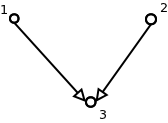
\includegraphics[scale=0.5]{./diagrams/bibliographic_coupling.png}
        \caption{Bibliographische Kopplung: Publikationen 1 und 2 sind bibliographisch gekoppelt, weil sie beide Publikation 3 zitieren}
        \label{fig:bibcoupling}
    \end{subfigure}
    \qquad
    \begin{subfigure}[h]{0.5\textwidth}
        \centering
        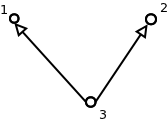
\includegraphics[scale=0.5]{./diagrams/co-citation.png}
        \caption{Kozitation: Publikationen 1 und 2 stehen in einer Kozitation-Relation zu einander, weil sie beide durch Publikation 3 zitiert werden}
        \label{fig:cocitation}
    \end{subfigure}
    \caption{Zitationsrelationen}
    \label{fig:citrelations}
\end{figure}
\\
\\
Eine andere Zitationsrelation ist die Kozitation.
Eine Kozitation von zwei oder mehreren Arbeiten liegt vor, wenn alle diese von einer dritten gemeinsam zitiert werden (Abbildung \ref{fig:cocitation}).
Laut Kim und Barnett \cite{DBLP:conf/amcis/KimB08} werden Cluster von h�ufig kozitierten Dokumenten als stark zusammenh�ngend betrachtet.
Auch Henry Small bezeichnet zwei Publikationen desto �hnlicher je �fter diese zusammen kozitiert werden \cite{Small_1973}.
% "Clusters of highly co-cited documents are considered to have high mutual dependance"\cite{DBLP:conf/amcis/KimB08}
\\
\\
\begin{figure}[h]
    \centering
    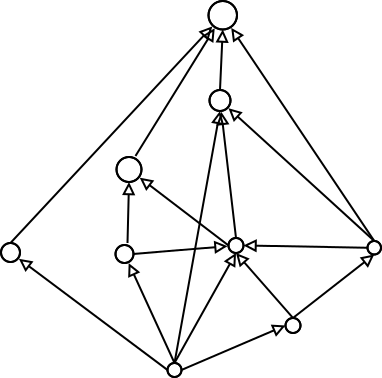
\includegraphics[scale=0.5]{./diagrams/citation_network.png}
    \caption{Beispiel f�r ein Zitationsnetzwerk}
    \label{fig:citenetwork}
\end{figure}
Aufgrund dieser beiden Auspr�gungen von Zitationsrelationen und auch noch der einfachsten und naheliegendsten: dem direkten Zitat, werden Zitationsnetzwerke aufgebaut.
Das sind Graphen, deren Knoten f�r Publikationen stehen und wo jede Kante eine Zitation veranschaulicht (Abbildung \ref{fig:citenetwork}).
Auf der Basis von Zitationsnetzwerken k�nnen Cluster von eng zusammenh�ngenden Dokumenten ermittelt werden.
Die gerichteten Kanten eines solchen Graphen stehen auch f�r eine zeitliche Richtung - das zitierte Paper ist stets �lter als die Arbeit, von der es zitiert wird.
Viele Experten schlagen �hnlichkeitsma�e vor, die auf Zitationsnetzwerken beruhen (siehe \cite{Small_1973}, \cite{Lu01nodesimilarity}, \cite{simrank2002}, \cite{ZhaoHS09} und \cite{DBLP:journals/corr/abs-1109-1059}).
\\
\\
Auch wenn diese bibliometrische Herangehensweise als ein sinnvoller erster Ansatz erscheint, um die �hnlichkeit zwischen zwei wissenschaftlichen Arbeiten zu ermitteln, werden bei n�herer Betrachtung mehrere Probleme/Kritikpunkte aufgedeckt, weswegen auf jeden Fall auch andere �hnlichkeitsindikatoren gesucht werden m�ssten:\\
\begin{itemize}
\item Selbstzitate: die Menschen tendieren dazu, sich selbst oder andere, die sie kennen und mit denen sie zusammen gearbeitet haben, �fters zu zitieren \cite{DBLP:conf/amcis/KimB08} \cite{frank2009einfuehrung}.
Dadurch versuchen sie einerseits ihre eigenen Parameter, wie z.B. Rankings aufgrund von Zitationszahlen, andererseits auch diese von Kollegen, Bekannten, etc. zu verbessern (die so genannten ``Dankbarkeits-'' oder ``Gef�lligkeitszitate'') \cite{DBLP:conf/isiwi/Schlogl00}.
Dazu kommt auch noch der Druck von Herausgebern von Journalen, dass Arbeiten, die in einem bestimmten Journal publiziert werden, m�glichst h�ufig andere Ver�ffentlichungen von diesem Journal zitieren (wieder aufgrund von Verbesserungen von bestimmten bibliometrischen Parametern) \cite{frank2009einfuehrung}.
\item Zitate von Standardwerken (sogenannten ``Authorities'') oder �bersichtsartikeln kommen vergleichsweise �fter vor und m�ssen mit Vorsicht genossen werden \cite{DBLP:conf/isiwi/Schlogl00} \cite{evalpubsim2005}.
\item Es dauert, bis sich eine Arbeit etabliert hat, deshalb werden fr�here Werke �fters zitiert \cite{DBLP:conf/isiwi/Schlogl00}.
\item Papers, die auf anderen Sprachen als Englisch ver�ffentlicht werden, werden tendenziell seltener gelesen und weniger zitiert \cite{Bornmann08}.
\item Manchmal werden Zitate einfach weggelassen \cite{DBLP:conf/isiwi/Schlogl00}.
\item Zwei Arbeiten, die eine Dritte zitieren, k�nnen sich wom�glich auf komplement�re Aspekte davon beziehen.
\item Artikel mit langen Referenzlisten sind tendenziell st�rker bibliographisch gekoppelt als solche mit kurzen Listen, wenn man nur die Anzahl der zusammen zitierten Arbeiten z�hlt \cite{frank2009einfuehrung}.
\item Zitate, die andere Arbeiten referenzieren, ohne das Originalwerk zu konsultieren: es werden in Bibliographien �fters Arbeiten aus dem Literaturverzeichnis eines zitierten Dokuments entnommen \cite{DBLP:conf/isiwi/Schlogl00}.
\item Rechtschreibfehler in Zitaten: aufgrund deren kann das zitierte Werk nicht eindeutig bestimmt/wiedergefundnen werden, was das Zitat wertlos macht \cite{Bornmann08}.
% Ansatz zur Normalisierung relative bibliographische Kopplung (Jaccard- und Salton-Index), messen die Kopplung bezogen auf die L�nge der Referenzlisten
\end{itemize}

\subsubsection{Koautorenschaft}

Der zweite Schwerpunkt, der hier noch kurz umrissen wird, ist die Koautorenschaft.
Als Koautoren werden zwei oder mehrere Wissenschaftler oder Wissenschaftlerinnen bezeichnet, die gemeinsam eine Arbeit ver�ffentlicht haben.
Koautorenschaft wird auch oftmals als ein �hnlichkeitskennzeichen gewertet \cite{Yang:2009:TRSN}. %Quelle!!
Allerdings hat die Definition eines �hnlichkeitsma�es, das auf Koautorenschaft alleine beruht, auch diverse Nachteile:\\
\begin{itemize}
\item Bei langen Autorenlisten sind manche Autorinnen nur teilweise im Thema involviert.
\item Der selbe Autor taucht oft unter verschiedenen Namen auf (Martin, J.; Martin, J.M.; Martin, James) \cite{DBLP:conf/isiwi/Schlogl00} \cite{Bornmann08}.
Deswegen ist es oft schwierig eindeutig einzuordnen, welche Person an der konkreten Publikation mitgearbeitet hat \cite{Yang:2009:TRSN}.
Dieses Problem ist noch st�rker ausgepr�gt, wenn die Namen der Autoren urspr�nglich im Kyrillischen oder einem anderen Alphabet geschrieben werden und ins lateinische Alphabet �berf�hrt werden m�ssen.
\item Es existiert auch das umgekehrte Problem:
Ein oft vorkommender Name, der sich auf verschiedene Personen bezieht, kann versehntlich aggregiert werden \cite{DBLP:conf/isiwi/Schlogl00} \cite{Bornmann08}.
% -> L�sung f�r die letzten 2: Benutzen eines eindeutigen Identifiers f�r jeden Autor (unser Datensatz hat das)
\end{itemize}

% Schlussfolgerung in die Richtung: deshalb brauchen wir andere Ans�tze, �hnlichkeit zu bestimmen

Zusammenfassend l�sst sich sagen, dass obwohl bibliometrische Analysen sich als ein erster Ansatz f�r �hnlichkeitsdefinition nutzen lassen, diese allein auf keinen Fall ersch�pfend sind und manchmal sogar zu falschen oder unbegr�ndeten Schlussfolgerungen f�hren k�nnen.
Zudem sind sie in manchen F�llen schwer anzuwenden.
Es ist kompliziert f�r Publikationen, die ihren Hauptschwerpunkt in verschiedenen Forschungsfeldern haben, nur aufgrund von Bibliometrie den �hnlichkeitsgrad zu bestimmen: unterschiedliche Disziplinen haben verschiedene Zitierungsgewohnheiten (in manchen wird viel zitiert, in manchen weniger) \cite{Bornmann08}, was die Arbeiten schwer vergleichbar macht.
% Pearsons Korrelationskoeffizient (wird auch oft f�r �hnlichkeitsmessungen verwendet)
% f�r jetzt lasse ichs erstmal


\subsection{Semantische Netzwerke}
In der heutigen globalisierten Welt wachsen die Mengen der verf�gbaren Informationen st�ndig exponentiell.
Deshalb ist eine geeignete Wissensrepr�sentation in jedem konkreten Fall der Informationsdarstellung und -verarbeitung besonders wichtig.
Diese sollte laut \cite{Bench-Capon:1990:KR} die folgenden Eigenschaften haben:\\
\begin{itemize}
\item eindeutig sein;
\item klar und konsistent sein;
\item ad�quat sein f�r die Ziele, f�r die sie gebraucht und eingesetzt wird;
\end{itemize}
Aus diesen Gr�nden modelliert die aktuelle Arbeit den Datensatz aus Publikationen und dazugeh�rigen Metadaten als ein semantisches Netz.
Ein semantisches Netz wird folgenderma�en charakterisiert \cite{Bench-Capon:1990:KR}:\\
\begin{itemize}
\item es besteht aus Entit�ten, die als Knoten modelliert werden
\item und Relationen zwischen diesen Entit�ten, die die Kanten des Netzes darstellen; die Kanten eines semantischen Netzes sind daher gelabeled;
\item es wird im Allgemeinen zwischen Klassen und Individuen, die zu einer bestimmten Klasse geh�ren, unterschieden;
\item Klassen und Individuen k�nnen Attribute haben;
\item die zu einem Objekt dazugeh�rigen Informationen werden in der N�he von diesem Objekt geclustert.
\end{itemize}
Jede Publikation und jedes dazugeh�rige Metadatum wird als ein Individuum modelliert.
Dabei werden die entsprechenden �bergeordneten Kategorien (Publikation, Autor, Quelle, Erscheinungsjahr u.s.w) als Klassen dargestellt.
Die zwischen einem Paper und seinen Metadaten bestehenden Relationen werden dann als die Kanten des semantischen Netzes repr�sentiert.
Aufgrund von dem so entstandenen Netzwerk mit Hilfe von graphentheoretischen Methoden sollen Publikationen auf �hnlichkeit verglichen werden.
Mehr zu der konkreten Modellierung wird in Kapitel 3.2 gesagt.

% Was sind semantische Netzwerke
% Warum sind sie in unserem Fall wichtig?/Warum haben wir uns f�r so eine Wissensrepr�sentation entschieden?
% (Wissensrepr�sentationen sollen die folgenden Eigenschaften haben: eindeutig sein; klar und konsistent sein; ad�quat f�r die Ziele, f�r die wir sie brauchen, sein; Rechnen drauf soll m�glich sein/sollen berechenbar sein

% das und das unten kommt aus \cite{Bench-Capon:1990:KR}


% Entit�ten als Knoten
% Relationen zwischen denen als Kanten
% Klassen vs Individuen
% Klassen und Individuen k�nnen auch Attribute haben
% Charakteristik: die Informationen zu einem bestimmten Objekt werden in der N�he von diesem Objekt geclustert

% und au�erdem (f�r Ontologien):
% Restriktionen
% Regeln
% Axiome
% Events

\subsection{Verwandte Arbeiten}
\subsubsection{Semantische Repr�sentation}
% Was gibt es schon zum Thema semantische Modellierung von Publikationen (Science Ontology, Diplomarbeit vom einen Typen\cite{abbildungXML2002} )
Matthias Erbarth schl�gt in seiner Diplomarbeit \cite{abbildungXML2002} eine semantische Modellierung mit Hilfe von XML-Technologien vor.
Diese bildet jedoch eine einzelne Publikation mit ihren Einzelteilen ab.
Das semantische Model einer Publikation soll dann mit einer Fachontologie in Verbindung gebracht werden, um eine ``erweiterte Stichwordindexierung'' zu erm�glichen.
Dabei liegt sein Schwerpunkt auf der Idee, dass indem das in einer wissenschaftlichen Arbeit enthaltene Wissen in einer maschinenlesbaren Form dargestellt wird, Aufgaben der Information Retrieval effizienter gel�st werden k�nnen.
% warum macht er das
% was n�tzliches/wichtiges erreicht er dadurch
% was f�r erkenntnisse kann man daraus f�r meinen fall ziehen
Die Ontology of Science von Fred Freitas \cite{ontosci} bildet eine ganze Dom�ne von Forschungseinrichtungen, -arbeiten, -prozessen, -ereignissen ab. %Abbildung!
Abbildung \ref{fig:ontosci} gibt einen �berblick �ber die Klassen dieser Ontologie.
Obwohl sie m�gliche Typen von wissenschaftlichen Publikationen ausf�hrlich in Form von Unterklassen abbildet, modelliert sie nicht alle zu einem wissenschaftlichen Dokument dazugeh�rigen Metadaten und die dazwischen bestehenden Relationen detailliert genug, um eine ad�quate Basis f�r den Entwurf eines semantischen �hnlichkeitsma�es f�r Publikationen aufgrund von Metadaten zu bieten.
Mehrere relevante Metadaten, wie Keywords, Klassifizierung, Zitationen, etc., werden von der Ontologie nicht modelliert.
Alle Unterklassen der Klasse \textit{Scientific Document} sind auf Abbildung \ref{fig:scientificdoc} dargestellt.
Auf Abbildung \ref{fig:scientificdoc_relations} sind die Relationen zwischen der Klasse \textit{Scientific Document} und anderen Klassen der Ontologie zu sehen.

\begin{figure}[hp]
    \centering
    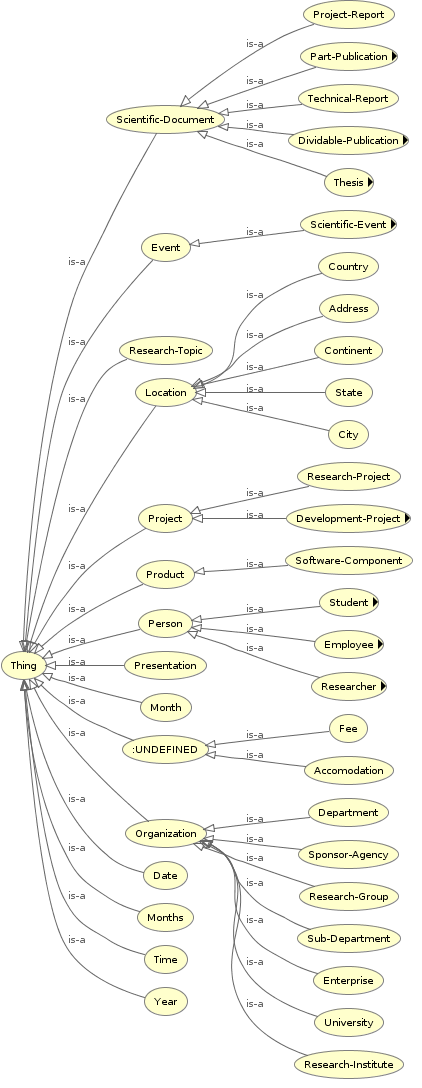
\includegraphics[scale=0.5]{../deps/ontology_of_science_complete_owlviz.png}
    \caption{Ontology of Science}
    \label{fig:ontosci}
\end{figure}

\begin{figure}[h!]
    \centering
    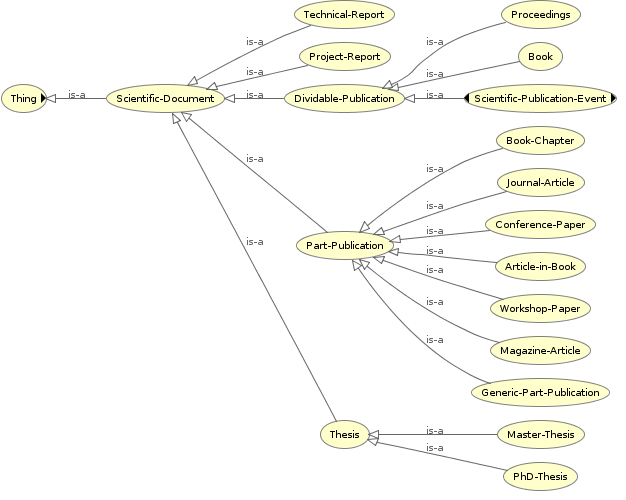
\includegraphics[scale=0.5]{../deps/ontology_of_science_scientificdoc_owlviz.png}
    \caption{Ontology of Science. Die Klasse \textit{Scientific Document}}
    \label{fig:scientificdoc}
\end{figure}

\begin{figure}[hp]
    \centering
    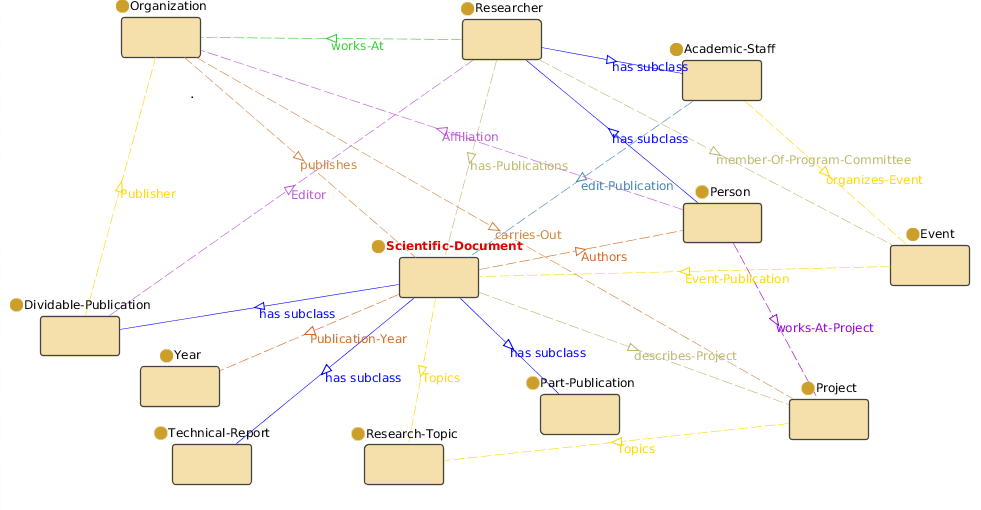
\includegraphics[angle=90,scale=0.5]{../deps/science_onto_scientific_doc3.png}
    \caption{Ontology of Science. Relationen zwischen \textit{Scientific Document} und anderen Klassen}
    \label{fig:scientificdoc_relations}
\end{figure}



\subsubsection{�hnlichkeitsma�e}
% Was gibt es schon zum Thema �hnlichkeitsma�en (Kozitationen, Koautorenschaften, bibliographische Kopplung,

% ----------- Textbasierte Ma�e -----------------------------------------------------------------------
Bani-Ahmad et al. unterscheiden in ihrem �bersichtsartikel \cite{evalpubsim2005} zwischen text- und zitationsbasierten �hnlichkeitsma�en f�r wissenschaftliche Publikationen.
Als Beispiel f�r ein textbasiertes Ma� nennen sie das auf die bekannte TF-IDF Metrik (Termfrequenz-Inverse Dokumentfrequenz) gest�tzte Kosinusma�.
Der TF-IDF-Wert eines Terms (oder Worts) ist proportional zur Anzahl der Vorkommen dieses Terms in einem Dokument und inversproportional zur Anzahl der Vorkommen des Terms im Gesamtkorpus.
Zwei Dokumente, deren �hnlichkeit bestimmt werden sollte, werden dann als Vektoren ihrer Termfrequenzen dargestellt.
Die Dokumente sind desto �hnlicher, je n�her zu einander sich diese Vektoren im Raum befinden, d.h. je kleiner der Winkel zwischen beiden ist (und je gr��er der Kosinus von diesem Winkel).
Dieses Ma� wird, in Kombination mit anderen Methoden, auch von den Erfindern der automatisierten Indexingdienst f�r wissenschaftliche Arbeiten CiteSeer\footnote{http://citeseerx.ist.psu.edu/index}, Lee Giles and Kurt D. Bollacker and Steve Lawrence, als �hnlichkeitsma� f�r Artikel eingesetzt \cite{Giles98citeseer}.
Mit Hilfe von dieser Metrik werden Titel, Inhaltsverzeichnis, Abstract und Volltext von Publikationen ausgewertet.
Der Ansatz ist aus mehreren Gr�nden problematisch.
Bei sehr gro�en Dokumentenmengen ist die Methode ziemlich rechenaufwendig.
Zudem ist diese sprachabh�ngig - es ist nicht m�glich aufgrund von reinen textbasierten Ma�en, wie dem Kosinusma� in Kombination mit TF-IDF, �hnlichkeit zwischen Artikeln, die auf verschiedenen Sprachen vorliegen, zu messen.
Au�erdem ist die semantische Bedeutung der Terme unbekannt, was die Ergebnisse verf�lschen kann (Negationen werden nicht als solche ber�cksichtigt, W�rter, die mehrere Bedeutungen haben, werden aggregiert) \cite{gottwaldrecommender} \cite{Giles98citeseer}.
% das Cosinusma� -- look for a paper!


% Evaluating Publication Similarity Measures \cite{evalpubsim2005}
% Es gibt 2 Arten von �hnlichkeitsma�en f�r Publikationen: textbasiert(Information Retrieval) und zitationsbasiert(Bibliometrie), die beiden Ans�tze liefern meistens auch ziemlich unterschiedliche Ergebnisse

% Textbasierte �hnlichkeitsma�e \cite{Giles98citeseer} und ...
% Nutzen TF-IDF (Term Frequency- Inversed Document Frequency) und Vektorraummodelle aus der Information Retrieval
% Mit diesen Ma�en werden Titel, Inhaltsverzeichnis, Abstract und Text von wissenschaftlichen Arbeiten ausgewertet
% Problematisch: bei Riesenumfangen, evtl unpraktisch
% Problem2: sprachenabh�ngig
% Problem3: semantische Bedeutung ist unbekannt, kann das Ergebnis verf�lschen (z.B. werden Negationen nicht als solche ber�cksichtigt) \cite{gottwaldrecommender}
% One limitation of this approach is the inherent noise  uncommon words may be shared by documents by coincidence, thereby giving false evidence that the documents are related.
% Another limitation of this approach is the ambiguity of words and phrases. For example "arm" could mean a human limb, or a weapon. Simple word frequencies do not differentiate these uses, requiring context analysis for separation. - related to Problem3

% ----------- Aufgrund von Links (linkbasierten/zitationsbasierte Ma�en)--------------------------------------------------
\smallskip
Die zweite gro�e Kategorie existierender �hnlichkeitsma�e f�r wissenschaftliche Publikationen beruht auf Zitationen.
Die Idee, dass Artikel, die gemeinsame Referenzen teilen, in irgendeiner Weise verwandt sind, ist auf M.M.Kessler \cite{Kessler:1963} zur�ckzuf�hren.
In seiner Arbeit ``Bibliographic coupling between scientific papers'' schl�gt er eine Methode f�r ``Gruppierung von technischen und wissenschaftlichen Papers aufgrund von bibliografischer Kopplung'' vor \cite{Kessler:1963}.
Der Erste, der explizit den Begriff \textit{�hnlichkeit} verwendet, ist Henry Small \cite{Small_1973}.
Im Gegensatz zu Kessler legt Small jedoch seinen Schwerpunkt nicht auf bibliografischer Kopplung, sondern auf Z�hlung von Kozitationen.
Er bezeichnet hohe Kozitationszahlen als einen Indikator f�r ``subject similarity'' und ``co-occurance of ideas''.
Kozitationenz�hlung als Methode f�r die Identifikation von Artikeln, die das selbe oder �hnliches Thema teilen, benutzen auch Kim und Barnett \cite{DBLP:conf/amcis/KimB08}.

\smallskip
Ein anderes zitationsbasiertes Ma� ist die \textit{Common Citation Inverse Document Frequency} (CC-IDF) \cite{Giles98citeseer}.
In Anlehnung an die TF-IDF, die einzelne Terme gewichtet, werden hier die Gewichte der Zitate bestimmt.
�hnlich wie bei TF-IDF geht CC-IDF davon aus, dass eine relativ seltene Zitation, die zwei Dokumente teilen, h�her gewichet werden sollte, als eine Zitation, die in vielen Papers vorkommt.

% Common Citation Inverse Document Frequency (CCIDF) \cite{Giles98citeseer}
% analogous to the word oriented TFIDF word weights
% As in the use of TFIDF, CCIDF assumes that if a very uncommon citation is shared by two documents, this should be weighted more highly than a citation made by a large number of documents.
% Algorithm:
% assign a weigth to each citation, equal to the inverse frequency of the citation in the entire database
% Determine list of citation and their weigths for document A and search the database for all the documents which share at least one citation with A
% For each of this documents determine the sum of the weigths of the shared with A citations
% sort the results

\smallskip
Das �hnlichkeitsma� \textit{SimRank} wurde 2002 von Jeh und Widom entworfen \cite{simrank2002}.
\textit{SimRank} misst allgemein die strukturelle �hnlichkeit von zwei Objekten in einem Netzwerk aufgrund von Links.
Die Autoren schlagen einen Algorithmus vor, der basierend auf dem Gesamtgraphen die �hnlichkeit zwischen zwei Knoten rekursiv berechnet.
Dabei gehen sie von der Leitidee ``zwei Objekte sind �hnlich, wenn sie mit �hnlichen Objekten verbunden sind'' \cite{simrank2002} aus.
Ferner erw�hnen sie, dass ein m�glicher Anwendungsbereich f�r ihr Ma� Zitationsgraphen sind, wo die strukturelle �hnlichkeit zwischen wissenschaftlichen Publikationen anhand von Literaturverweisen rekursiv bestimmt werden kann.

Zhao, Han und Sun haben mit \textit{P-Rank} ein �hnliches Konzept \cite{ZhaoHS09}.
\textit{P-Rank} ist ebenso ein strukturelles �hnlichkeitsma� f�r Informationsnetzwerken, unterscheidet sich jedoch von \textit{SimRank} durch die Tatsache, dass es nicht nur ein- sonder auch ausgehende Kanten in die �hnlichkeitsberechnung miteinbezieht.
Es verallgemeinert das zugrundeliegende Prinzip von \textit{SimRank} folgenderma�en: ``zwei Objekte sind �hnlich, wenn sie (1) durch �hnliche Objekte referenziert werden; und (2) �hnliche Objekte referenzieren'' \cite{ZhaoHS09}.
Die Autoren argumentieren, dass bibliografische Kopplung, Kozitationen und \textit{SimRank} lediglich Spezialf�lle von \textit{P-Rank} sind.
%auch Amsler wenn sich das Originalpaper findet.
% die Tabelle, die alle zusammenfasst!!
Das Gemeinsame zwischen \textit{SimRank} und \textit{P-Rank} ist die Propagierung der �hnlichkeitswerte �ber das gesamte Netzwerk und die rekursive Art ihrer Berechnung.
Eine Verbesserung von \textit{P-Rank} gegen�ber \textit{SimRank} ist die M�glichkeit, �hnlichkeitswerte f�r neuere und potentiell interessante, aber immer noch nicht popul�re Arbeiten zu ermitteln.
\textit{SimRank}, das nur eingehende Kanten ber�cksichtigt, kann das nicht leisten.

% Arbeiten, die (unter anderem) auch �hnlichkeit von Papers berechnen,
% Aber NUR auf Grund von Zitationen

% P-Rank: a Comprehensive Structural Similarity Measure over Information Networks \cite{ZhaoHS09}
% guckt sich sowohl homogene als auch heterogene netze an, misst aber �hlichkeit nur zwischen entit�ten, die zur selben kategorie geh�ren
% we consider an entity maximally similar to itself, to which we can assign the P-Rank score of 1. (If other entities are known to be similar a-priori, their similarities can be pre-assigned as well.)

% Small 1973: --- Argument daf�r, dass beides ber�cksichtigen Sinn macht!!
% co-citation patterns are found to differ significantly from bibliographic coupling patterns, but to agree generally with patterns of direct citation
% absence of any clear relationship between bibliographic coupling strength and co-citation frequency
% based on this example one might be tempted to hypothesize that co-citation, like bibliographic coupling, measures subject similarity. However, the same agreement between bibliographic coupling and co-citation strength was not observed in other cases.
% Small hat beobachtet, dass Gruppierungen von ``�hnlichen'' Papers aufgrund von Kozitationen und bibliografischer Kopplung zu sehr unterschiedlichen Resulaten f�hren.

Angelehnt an \textit{SimRank} und \textit{P-Rank} schlagen Yoon, Kim und Park das linkbasierte �hnlichkeitsma� f�r wissenschaftliche Literatur \textit{C-Rank} vor \cite{DBLP:journals/corr/abs-1109-1059}.
Sie geben selber nochmal einen �berblick �ber schon vorhandene �hnlichkeitsma�e f�r wissenschaftliche Arbeiten und z�hlen gleichzeitig auch ihre Schw�chen auf:\\
\begin{itemize}
\item Textbasierte Metriken f�r �hnlichkeitsbestimmung wissenschaftlicher Publikationen w�rden zwei Papers auch dann als �hnlich bezeichnen, wenn sie demselben Forschungsfeld angeh�ren, auch wenn sie sich mit unterschiedlichen Problemen besch�ftigen.
\item Die bibliografische Kopplung ist ungeeignet, um �hnlichkeit zwischen alten aber �hnlichen Arbeit zu berechnen.
\item Durch Kozitationz�hlung kann die �hnlichkeit zwischen neuen �hnlichen Arbeiten nicht gemessen werden.
\item Beide sind nicht in der Lage �hnlichkeit zwischen einem alten und einem neuen Paper, die �hnlich sind, zu bestimmen. Die alte Arbeit zitiert keine Neueren, die Neue kann nicht durch �ltere zitiert werden.
\item \textit{SimRank}, das in gewissem Sinn eine Generalisierung der Kozitation ist, kann keine �hnlichkeit berechnen, wenn ein Paper durch keine Anderen zitiert wird.
\item Es wird noch \textit{rvs-SimRank} (reverse SimRank) genannt, das im Gegensatz zu \textit{SimRank} nur ausgehende Links f�r seine Berechnung betrachtet.
Demzufolge hat dieses Ma� auch den Nachteil, dass es keine �hnlichkeit bestimmen kann, wenn ein Paper keine Anderen zitiert.
\item \textit{P-Rank} betrachtet sowohl ein- als auch ausgehende Kanten, ist aber auch f�r Bestimmen der �hnlichkeit zwischen einer alten und einer neuen Arbeit ungeeignet.
\end{itemize}
�hnlich wie \textit{P-Rank} st�tzt sich \textit{C-Rank} gleichzeitig auf ein- und ausgehenden Kanten.
Dabei ist der Unterschied zwischen beiden Ans�tzen, dass \textit{P-Rank} eine geeignete Gewichtung beider Arten von Kanten vornimmt und \textit{C-Rank} �berhaupt nicht dazwischen unterscheidet.
\textit{C-Rank} geht tats�chlich aus einem ungerichteten Zitationsgraphen aus.
Die Autoren haben in ihrer Evaluation festgestellt, dass sie dadurch in der Lage sind, �hnlichkeit zwischen alten und neuen Arbeiten zu bestimmen, was keinem anderen der zitationsbasierten �hnlichkeitsma�e gelungen war.

\smallskip
Eine etwas unterschiedliche Herangehensweise w�hlen Lu et al. in ihrer Definition von Knoten�hnlichkeit in Informationsnetzwerken \cite{Lu01nodesimilarity}.
Diese l�sst sich, genau wie alle anderen bereits erw�hnten strukturellen �hnlichkeitsma�e, auf Zitationsgraphen von wissenschaftlichen Publikationen anwenden.
Genauer gesagt, arbeiten Lu und seine Kollegen zwei verschiedene Ma�en aus.
Beide beziehen (im Gegensatz zu \textit{SimRank}, \textit{P-Rank} und \textit{C-Rank}) nur die lokale Nachbarschaft von Knoten in die �hnlichkeitsberechnung ein.
Das erste Ma�, das die Forscher vorschlagen, basiert auf dem Vergleich der separaten lokalen Nachbarschaften von zwei Knoten.
Jedem Knoten wird ein Authority-Gewicht zugewiesen.
Zwei Knoten sind dann desto �hnlicher, je gr��er der Schnitt deren lokalen Nachbarschaftsgraphen ist und je mehr Authority-Papers in diesem Schnitt liegen.
Der zweite Ansatz beruht auf der Berechnung des Netzwerkflusses. %Network flow??
Er ermittelt wie stark zwei Publikationen in einem Zitatiosgraphen miteinander verbunden sind.
Daf�r wird der gemeinsame lokale Nachbarschaftsgraph zweier Publikationen aufgebaut.
Der \textit{Maximum Flow Minimum Cut} Algorithmus \cite{chinneck2010} wird benutzt um den Fluss auszurechnen, der vom einen zum anderen Knoten gereicht werden kann.
%Es werden die verschiedenen Pfade zwischen beiden Knoten gez�hlt.
%Dabei tragen l�ngere Pfade weniger zu der �hnlichkeit zwischen den Knoten bei.
%Der Minimum Cut bestimmt die Anzahl der Kanten, die entfernt werden sollten, um beide Knoten komplett von einander zu trennen.


%----------------------------------------------------------------------------------------------------------------
% A slightly different approach: Node similarity in neworked information spaces \cite{Lu01nodesimilarity}
% 1):
%  based on a comparison of subgraphs based on hubs and authority values
% measures how similar the both local citation communities are
% uses vectors to compute similarity; authority weight is assigned to every node; two papers are similar if their individual local citation graphs share similar authority papers
% construct two separate local citation graphs
% two papers are probably more similar to each other if they are connected by reference coupling or co-citation by authority papers than by hubs
% in order to get high similarity between papers their graphs must have a large intersection and there must be many authority papers in the intersection area
% uses authority weigth as a measure of importance
%
% 2):
% based on a network flow computation
%  how strongly the two papers are connected in the citation graph
% uses maximus flow/minimum cut algorithm to compute the amount of flow which can be pushed from one paper to another
% key idea: count the number of different paths between the two papers
% minimum cut: the minimum number of edges which needs to be cut in order to disconnect the one paper from the other
% longer paths are less indicative for similarity than shorter ones
% more links: higher capacity for link between source and sink, more links need to be cut in order to disconnect source from sink
% an edge which is far away from the source/sink paper gets a low capacity weight, therefore you cannot push more flow through a longer path and as a result a longer path will contribute less to the overall flow from source to sink
% the similarity metric should give the same value for two adjacent nodes as for two non-adjacent nodes, who have d common neighbours

Yang et al. pr�sentieren mit ihrer Arbeit \cite{Yang:2009:TRSN} ein �hnlichkeitsma� f�r Autoren wissenschaftlicher Literatur.
Das Interessante an dem Entwurf ist, dass er, im Gegensatz zu allen zitationsbasierten Ma�en f�r Publikationen, verschiedene Metadaten in die �hnlichkeitsberechnung miteinbezieht.
Die Wissenschaftler bestimmen die �hnlichkeit zwischen Autoren anhand mehrerer Daten:\\
\begin{itemize}
\item Keywords, die die Forschungsschwerpunkte der Autoren beschreiben,
\item der pers�nlichen Interessen der Autoren (diese werden von den Autoren selbst formuliert oder aus deren Webseiten extrahiert),
\item Themen der Konferenzen, die die Autoren besuchen,
\item Koautorenschaften.
\end{itemize}
Diese Ans�tze werden sowohl einzeln als auch gewichtet zusammen angewandt.
Die Arbeit kommt zu der Schlussfolgerung, dass eine gewichtete Summe die �hnlichkeit am pr�zisesten bestimmt und zudem dass Ergebnisse, die nur aufgrund von Keywords erzielt worden sind, genauer sind als solche, die auf Koautorenschaften basieren.

% �hnlichkeit zwischen Autoren: \cite{Yang:2009:TRSN}) --- das interessante ist, dass sie Metadaten in die Auswertung miteinbeziehen
% Ziel vom Paper: Modellierung eines sozialen Netzwerkes von Autoren
% Haben mehrere Methoden genutzt und mit einander verglichen: anhand von Schl�sselw�rtern/Keywords, anhand von den pers�nlichen Interessen der Autoren (von den Autoren selber bestimmt/aus deren Webpages extrahiert), anhand von Themen der Konferenzen, wo Autoren hingehen/Papers ver�ffentlichen, anhand von Koautorenschaften;
% Die Methoden wurden sowohl einzeln angewandt als auch gewichtet zusammen
% Keywords basierte Graphen wurden von den Autoren selber als aussagekr�ftiger gewertet als solche, die auf Koautorenschaften basierten
% Probleme, wenn man nur Koautoren nutzt (siehe oben in der Beschreibung von Bibliometrie)
% Probleme, wenn man Keywords nutzt: das selbe Keyword kann unterschiedlich geschrieben werden (web2.0 vs Web 2.0); hat den Nachteil, dass die Untersuchten Papers auf der selben Sprache sein sollten (bei uns sind English Keywords im Datensatz definiert, es kann aber nicht immer auf die H�ufigkeit dieser im Volltext zur�ckgegriffen werden; wobei das werde ich vermutlich auch gar nicht tun)

Dieser �berblick zeigt die Vor- und Nachteile schon vorhandener �hnlichkeitsma�e.
Alle strukturellen Ans�tze, die nur auf Zitationen basieren, ber�cksichtigen in ihrer �hnlichkeitsberechnung nur eine Art von vielen m�glichen Metadaten.
Ferner sind Zitationen alleine kein aussagekr�ftiger Indikator f�r �hnlichkeit, da wissenschaftliche Arbeiten andere Publikationen aus verschiedenen Gr�nden zitieren k�nnen.
Diese gemeinsame Schw�che l�sst darauf schlie�en, dass wir eine neue, allgemeinere Definition von �hnlichkeit brauchen.

% Aus diesen Gr�nden brauchen wir eine neue, allgemeinere Definition von �hnlichkeit.

\newtheorem{mydef}{Definition}
\textbf{�berblick �ber die schon vorhandenen zitationsbasierten �hnlichkeitsma�e f�r Publikationen}
\\
\begin{mydef}[Bibliographische Kopplung]
\[
sim(a,b) = O(a) \cap O(b)
\]
\newline
%Frage: schl�gt er auch Normalisierung vor?
\newline
Die Anzahl der gemeinsamen ausgehenden Links
\end{mydef}


\begin{mydef}[Kozitation]
\[
 sim(a,b) = I(a) \cap I(b)
\]
\newline
% Normalisierung?
Die Anzahl der gemeinsamen eingehenden Links
\end{mydef}

\begin{mydef}[Amsler]
\[
 sim(a,b) = \cfrac{L(a) \cap L(b)}{L(a) \cup L(b)}
\]
\newline
Die Anzahl der gemeinsamen Links.
(Sowohl ein- als auch ausgehende Links werden gez�hlt.
Eine Unterscheidung zwischen beiden Arten von Links unternimmt Amsler nicht.)
Das Ergebnis wird normalisiert, indem es durch die Anzahl aller Links beiden Publikationen geteilt wird.
\end{mydef}


\begin{mydef}[SimRank]
\[
sim(a,b) = 1 \quad \text{wenn } a=b
\]
\newline
\text{sonst}
\[
sim(a,b)  = 
        \cfrac{c}{|I(a)||I(b)|}
        \sum_{i=1}^{|I(a)|} \sum_{j=1}^{|I(b)|} sim(I_i(a),I_j(b))
\]
\newline
\end{mydef}

\begin{mydef}[rvs-SimRank]
\[
sim(a,b) = 1 \quad \text{wenn } a=b
\]
\newline
\text{sonst}
\[
sim(a,b)  = 
        \cfrac{c}{|O(a)||O(b)|}
        \sum_{i=1}^{|O(a)|} \sum_{j=1}^{|O(b)|} sim(O_i(a),O_j(b))
\]
\newline
\end{mydef}


\begin{mydef}[P-Rank]
\[
sim(a,b) = 1 \quad \text{wenn } a=b
\]
\newline
\text{sonst}
\[
\begin{array}{lcl}
sim(a,b) & = &
        \lambda\times\cfrac{c}{|I(a)||I(b)|}
        \sum_{i=1}^{|I(a)|} \sum_{j=1}^{|I(b)|} sim(I_i(a),I_j(b))
        \\ & + &
        (1-\lambda)\times\cfrac{c}{|O(a)||O(b)|}
        \sum_{i=1}^{|O(a)|} \sum_{j=1}^{|O(b)|} sim(O_i(a),O_j(b))
\end{array}
\]
\newline
\end{mydef}


\begin{mydef}[C-Rank]
\[
sim(a,b) = 1 \quad \text{wenn } a=b
\]
\newline
\text{sonst}
\[
sim(a,b)  = 
        \cfrac{c}{|L(a)||L(b)|}
        \sum_{i=1}^{|L(a)|} \sum_{j=1}^{|L(b)|} sim(L_i(a),L_j(b))
\]
\newline
\end{mydef}

Tabelle \ref{tab:compareMeasures}\footnote{Tabelle \ref{tab:compareMeasures} ist mit einigen Modifikationen aus \cite{ZhaoHS09} �bernommen worden. Dabei ist noch zu bemerken, dass Zhao, Han und Sun das \textit{Amsler-Ma�} f�lschlicherweise in die Spalte \textit{``Beide, gewichtet''} kategorisiert haben. Amsler selber betrachtet zwar sowohl ein- als auch ausgehende Links, macht aber keine Unterscheidung dazwischen und demzufolge auch keine Gewichtung \cite{amsler1972applications}.} fasst nochmal die existierenden �hnlichkeitsma�e zusammen.
In der Zeile \textit{``Lokal''} stehen diejenigen Ma�e, die nur die lokale Nachbarschaftien von 2 Publikationen f�r das Bestimmen ihrer �hnlichkeit einbeziehen.
In der Zeile \textit{``Global''} dagegen befinden sich die Ma�e, die bei der Berechnung der �hnlichkeit von zwei Papers das gesamte Publikationsnetzwerk rekursiv betrachten.
Dabei ist $k$ die Anzahl der Iterationen, die jedes Ma� verwendet,
$c$ ist das benutzte D�mpfungsfaktor,
$\lambda$ ist der Parameter, der die Gewichtung der eingehenden Zitationen bestimmt.
(wenn $\lambda=1$ werden nur eingehende Links ber�cksichtigt, wenn $\lambda=0$ werden nur ausgehende Links ber�cksichtigt.)
In der Spalte \textit{``Beide, gewichtet''} stehen die Ma�e, die sowohl ein- als auch ausgehende Link in einer bestimmten Gewichtung in ihrer Berechnung miteinbeziehen.
In der Spalte \textit{``Beide, keine Gewichtung''} stehen Ma�e, die auch beide Arten von Links miteinbeziehen, allerdings ohne zwischen diesen Arten zu unterscheiden.

\begin{table}[h]
\centering
\begin{tabular}{| m{2cm} | m{2cm} | m{2cm} | m{2.5cm} | m{2cm} |}
    \hline
    \textbf{} & \textbf{In-Link} & \textbf{Out-Link} & \textbf{Beide, gewichtet} & \textbf{Beide, keine \newline Gewichtung}\\
    \hline
    Lokal \newline $k=1, c=1$ & Kozitation \newline $\lambda=1$ & Kopplung \newline $\lambda=0$ & & Amsler \newline kein $\lambda$\\
    \hline
    Global \newline $k=\infty$, \newline $c=variiert$ & SimRank \newline $\lambda=1$ & rvs-SimRank \newline $\lambda=0$ & P-Rank \newline $\lambda=variiert$ & C-Rank \newline kein $\lambda$ \\
    \hline
\end{tabular}
\caption{Existierende �hnlichkeitsma�e in Vergleich}
\label{tab:compareMeasures}
\end{table}


\newpage
\section{Entwurf und Implementierung}
\subsection{Analyse des zugrundeliegenden Datensatzes}
%Erklaerung was das Zentralblatt Mathematik ist - siehe homepage
lalalal
\subsection{Modellierung des semantischen Netzes}

\subsection{Mapping auf das entworfene Schema}

\subsection{Ein �hnlichkeitsma� f�r mathematische Publikationen}

\newpage
\section{Evaluation}

\subsection{Testl�ufe}
%Um das vorgeschlagene �hnlichkeitsma� f�r wissenschaftliche Publikationen auswerten zu k�nnen, wird der Testdatensatz vom Zentralblatt Mathematik auf das im Kapitel \ref{subsec:modell} vorgestellte Graphenschema abgebildet.
%Mit Hilfe von einem in \textit{Python} geschriebenen Parser werden die Daten vom \textit{zmath}-Datensatz in \textit{GraphML}-Format �berf�hrt.
%Die \textit{GraphML}-Repr�sentation der vollst�ndigen Daten ist ca. $4.8$ Gb gro�.



% Anwendung des �hnlichkeitsma�es
% Was hats gebracht/wie siehts aus?

% Parameters of the test system:
%Hardware Overview:
%    Model Name: Mac Pro
%    Model Identifier: MacPro4,1
%    Processor Name: Quad-Core Intel Xeon
%    Processor Speed: 2,93 GHz
%    Number Of Processors: 2
%    Total Number Of Cores: 8
%    L2 Cache (per core): 256 KB
%    L3 Cache (per processor): 8 MB
%    Memory: 14 GB
%    Processor Interconnect Speed: 6.4 GT/s

%System Software Overview:
%    System Version: Mac OS X 10.6.8 (10K549)
%    Kernel Version: Darwin 10.8.0
%    Boot Volume: Macintosh HD
%    Boot Mode: Normal

% wie werden die lambdas gew�hlt? warum?
% wie wird c gew�hlt? warum (simRank optimierungspaper)

% Notes on accuracy, decay factor and convergence:
% ------------------------------------------------

% Accuracy: C-Rank > SimRank > P-Rank > rvs-SimRank

% Number of iterations:
% SimRank converges at k = 3,
% rvs-SimRank converges at k = 5,
% P-Rank converges at k = 6,
% C-Rank converges at k = 9.

% Decay factor:
% It is obvious that the similarity score of C-Rank increases with the increase of C.
% When C = 0.2, C-Rank converges fast at k = 2.
% When C = 0.8, on the other hand, C-Rank converges at the 9-th iteration.
% When C is low, the recursive power of C-Rank is weakened such that only the papers in local or near-local neighborhood are used in similarity computation.
% When C is high, more papers in a more global neighborhood can be used in computing the similarity recursively. When C is high, therefore, the convergence takes more time.

\subsection{Auswertung der Ergebnisse}
% Macht das, was rauskommt, Sinn?

% Vergleich gegen die MSC-Klassen
% Vergleich mit einem rein bibliometrischen Verfahren (bibliographische Kopplung / SimRank/ ..)
% Entwickle 3 Varianten und vergleich sie: mit unterschiedlichen Gewichtung von den verschiedenen Relationen
% Idee dahinter: wenn alle Relationen gleich gewichtet sind, dann k�nnen wir genau so gut auch keinen Unterschied zwischen denen machen
% Aber wir k�nnen die gleichgewichtete Variante als eine von den 3 nehmen

% evaluiere Performance (Zeit, Platz, ..)

% vgl mit den anderen Ma�en (SimRank, P-Rank, C-Rank): auf wie vielen Daten wurden diese angewandt? Wie viele Ressourcen hat die Berechnung in Anspruch genommen?

% Datensatz trimmen: weil so lange
% Klar machen nach welchem Prinzip getrimmt wird und was die Nachteile davon sind (Relationen gehen verloren)
% Andererseits wenn nur fr�here Publikationen betrachtet werden, werden zumindest keine Zitationsrelatioonen zu sp�teren Papers verloren
% Trimmen ist trotzdem schei�e, weil sich Zitationsverhalten so wie die Tendenzen zu gr��eren Koautorenschaften  mit der Zeit ver�ndert
% klar machen dass der Algorithmus in Zeit O(n^4) l�uft und warum (Pseudocode)

\newpage
\section{Zusammenfassung}


Diese Arbeit hat ein rekursives semantisches �hnlichkeitsma� f�r ein Informationsnetzwerk von wissenschaftlichen Publikationen und ihren Metadaten entworfen und implementiert.
Innerhalb des Netzwerkes wurden Publikationen sowie die vorhandenen Metadaten als Knoten modelliert.
Zur Evaluation des entwickelten Ma�es wurde ein Clusterverfahren auf die berechneten �hnlichkeitswerte angewandt und mit im Datensatz vergebenen MSC-Klassen mit dem Ziel verglichen, dass �hnliche Publikationen auch in �hnliche MSC-Klassen geh�ren.
Das �hnlichkeitsma� und anschlie�end das Clusterverfahren wurde auf einen Testdatensatz aus $3095$ ausgew�hlten Publikationen des \textit{Zentralblatt Mathematik} angewandt.
Das entwickelte Ma� ist unter der Annahme entstanden, dass zwei Publikationen �hnlich sind, wenn sie innerhalb des Netzwerks �ber �hnliche Metadaten verbunden sind.
\\
\\
Die experimentellen Ergebnisse des Clusterverfahrens haben gezeigt, dass sich das semantische �hnlichkeitsma� besser f�r die �hnlichkeitsberechnung zweier Publikationen eignet als das strukturelle Ma� \textit{C-Rank}, das nur auf Zitationen basiert.
\textit{C-Rank} ist nicht in der Lage, brauchbare �hnlichkeitswerte zu liefern, wenn keine vollst�ndige Referenzlisten der untersuchten Publikationen vorliegen.
Das entwickelte Verfahren hingegen verwendet auch andere Metadaten, die weitere wichtige Informationen �ber die wissenschaftlichen Arbeiten liefern.
Diese sollten bei einer �hnlichkeitsanalyse der Publikationen nicht vernachl�ssigt werden.
\\
\\
Das Verfahren hat, wie andere verwandte Ans�tze auch, eine sehr komplexe Laufzeit.
Dadurch war es im Rahmen dieser Arbeit leider nicht m�glich, das Verfahren auf dem kompletten \textit{zmath}-Datensatz zu testen.


\subsection{Ausblick}
Das in dieser Arbeit vorgeschlagene semantische �hnlichkeitsma� kann in verschiedenen Richtungen optimiert und weiterentwickelt werden.
\\
\\
Wie auch durch die Evaluation bekr�ftigt, ist es von entscheidender Bedeutung, dass die semantische �hnlichkeit f�r einen gesamten, nicht verkleinerten Datenatz berechnet wird.
Ein Nachteil des entworfenen Algorithmus, der seine Anwendung auf gro�e Datenmengen ma�geblich erschwert, ist seine Laufzeitkomplexit�t $\mathcal{O}(n^4)$.
Eine wertvolle Optimierung w�re die Parallelisierung der Berechnungen.
Die Frage, ob der Algorithmus parallelisierbar ist, ist offen und muss n�her untersucht werden.
\cite{Li2010} schlagen ein nicht iteratives Verfahren f�r die Berechnung von \textit{SimRank} vor, das die Berechnung der �hnlichkeiten wesentlich beschleunigt.
Es scheint leider in seiner urspr�glichen Form nicht anwendbar f�r die Berechnung der semantischen �hnlichkeit in einem heterogenen Publikationsnetzwerk, das verschiedene Arten von Knoten beinhaltet.
Die M�glichkeit, ein nicht iteratives Verfahren f�r die Berechnung der semantischen �hnlichkeit, das auf \cite{Li2010} basiert, zu entwickeln, kann untersucht werden.
\\
\\
Eine andere Erweiterung des vorgeschlagenen Algorithmus f�r semantische �hnlichkeit w�re die Ber�cksichtigung weiterer verf�gbarer Metadaten wie z.B. Titel oder Abstract.
Der Algorithmus kann dann mit textbasierten �hnlichkeitsmetriken, die die �hnlichkeit von Titel und Abstract zweier Publikationen ermitteln k�nnen, kombiniert werden.
Dar�ber hinaus k�nnen bei mathematischen Publikationen auch zus�tzliche Komponenten wie Formeln, Theoreme oder Diagramme in das �hnlichkeitsma� miteinbezogen werden.
Das entwickelte Verfahren besitzt also ausreichend Potential zur Weiterentwicklung.

%nochmal betonen, dass durch trimming informationen verloren gehen
% bessere rechner, mehr zeit wird gebraucht
% optimieren des algorithmus? parallelisieren
%% publikationsnetzwerk auslagern, nur �hnlichkeitsmatrix im arbeitsspeicher
%% wenn G zu gro�, kann mans extern, au�erhalb des Hauptspeichers auslagern (z.b. Graphdatenbank) (die �hnlichkeitsmatrix, egal welche Struktur f�r ihre Repr�sentation gew�hlt wird, wird erstmal einfachshalber im Arbeitsspeicher behalten
% das eigentliche (gr��ere) Problem ist die Laufzeit -- es k�nnen Verfahren gesucht werden, um die zu optimieren / Teile des Algorithmus zu parallelisieren
% anderer ansatz, der das gesamte netzwerk betrachet (und alle metadaten)

% vlt andere daten miteinbeziehen: den ansatz mit einem textbasierten f�r title/abstract kombinieren
% vlt auch formeln, theoreme, diagramme auswerten



%----------------------------------------------
%* was haben wir gemacht
%* was gewinnen wir durch semantische Analyse von Metadaten
%* hinweis auf weiterf�hrende recherche

% Koennen wir auch weitere Daten analysieren? Auf anderen Weisen (nicht semantisch)?
% zb mathematische formeln/theoreme/diagramme, die im text vorkommen
% Wie kann man das �hnlichkeitsma� anders/besser definieren?

% man kann das semantische �hnlichkeitsma� mit einem textbasierten kombinieren, das die �hnlichkeit zwischen Title/Abstracts auswertet, und diese dann auch f�r die Semantische �hnlichkeit nutzen
% Levenshtein distance: einfache Distanz zwischen 2 Strings/Texten \cite ???
% basiert auf die Anzahl von Einf�gungen, L�schungen, Ersetzungen von Buchstaben, die gebraucht werden, um einen String in einen anderen zu transformieren
% extrem unpraktisch: wir k�nnen nicht f�r tausende von Dokumenten, mit mehreren Seiten Text die Levenshteindistanz messen..
% fragw�rdig, ob brauchbare Ergebnisse rauskommen (wobei man k�nnte vlt so was schon f�r das Bauen einer Plagiatsoftware einsetzen..)
% kann vlt f�r das vergleichen von Abstracts/Titel genutzt werden


% man kann doch als weiterf�hrende Forschung eben solche Anwendungen bauen, die auf so einem �hnlichkeitsma� beruhen
% man kann das Ma� auch daf�r nutzen, zeitliche Analyse der Entwicklung der Wissenschaft in bestimmten Forschungsfelder/zu bestimmten Forschungsthemen zu entwerfen


%In a general way,
%
%restate your topic and why it is important,
%restate your thesis/claim,
%address opposing viewpoints and explain why readers should align with your position,
%call for action or overview future research possibilities.
%
%from my specific topic to more general matters
%say what you have already said but do it quickly, sharply and in different words


%--------------------------------------------------------
%----Literatur-------------------------------------------
%--------------------------------------------------------

\nocite{*}
%\nocite{HasChe11}
%\nocite{DBLP:journals/jmlr/HahslerCHB11}
%\nocite{HahGruHorBuc11}
\newpage

\bibliographystyle{lni}
\bibliography{vorl-literatur}

\end{document}
